\documentclass{standalone}
\usepackage{tikz}
\usetikzlibrary{patterns, positioning}
\usepackage[sfdefault]{ClearSans} %% option 'sfdefault' activates Clear Sans as the default text font
\usepackage[T1]{fontenc}

\begin{document}
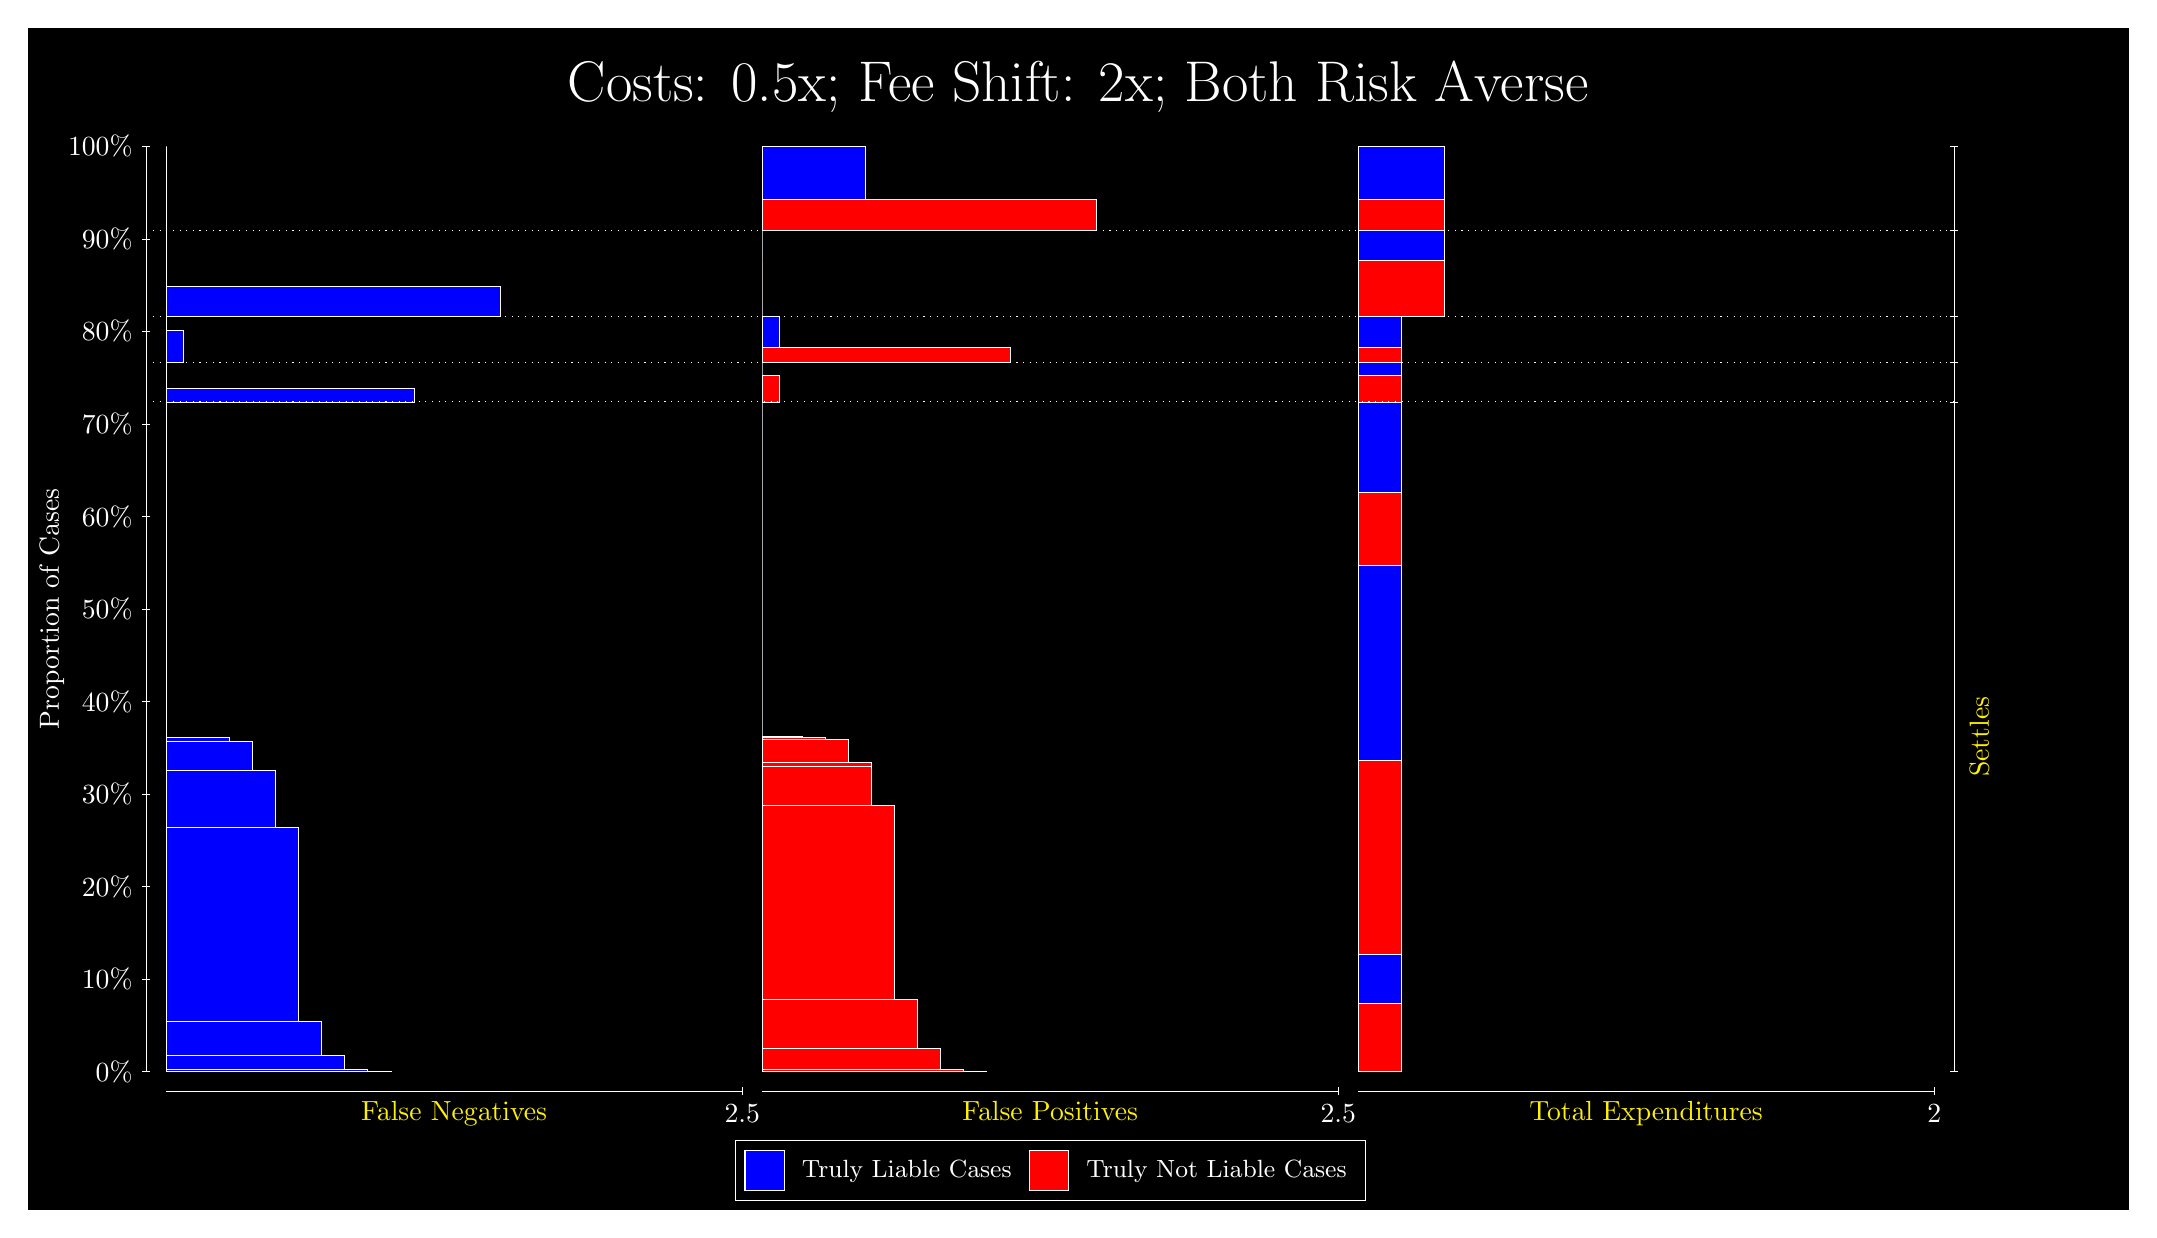
\begin{tikzpicture}
\draw[fill=black] (0,0) rectangle (26.667,15);
\draw[text=white] (0,13.5) rectangle (26.667,15) node[midway] {\huge Costs: 0.5x; Fee Shift: 2x; Both Risk Averse};
\draw[white, very thin] (1.5,1.75) -- (1.5,13.5);
\node[rotate=90, text=white, anchor=center] at (0.3, 7.625) {Proportion of Cases};
\draw[white, very thin] (1.45,1.75) -- (1.55,1.75);
\node[text=white, anchor=east] at (1.45, 1.75) {0\%};
\draw[white, very thin] (1.45,2.925) -- (1.55,2.925);
\node[text=white, anchor=east] at (1.45, 2.925) {10\%};
\draw[white, very thin] (1.45,4.1) -- (1.55,4.1);
\node[text=white, anchor=east] at (1.45, 4.1) {20\%};
\draw[white, very thin] (1.45,5.275) -- (1.55,5.275);
\node[text=white, anchor=east] at (1.45, 5.275) {30\%};
\draw[white, very thin] (1.45,6.45) -- (1.55,6.45);
\node[text=white, anchor=east] at (1.45, 6.45) {40\%};
\draw[white, very thin] (1.45,7.625) -- (1.55,7.625);
\node[text=white, anchor=east] at (1.45, 7.625) {50\%};
\draw[white, very thin] (1.45,8.8) -- (1.55,8.8);
\node[text=white, anchor=east] at (1.45, 8.8) {60\%};
\draw[white, very thin] (1.45,9.975) -- (1.55,9.975);
\node[text=white, anchor=east] at (1.45, 9.975) {70\%};
\draw[white, very thin] (1.45,11.15) -- (1.55,11.15);
\node[text=white, anchor=east] at (1.45, 11.15) {80\%};
\draw[white, very thin] (1.45,12.325) -- (1.55,12.325);
\node[text=white, anchor=east] at (1.45, 12.325) {90\%};
\draw[white, very thin] (1.45,13.5) -- (1.55,13.5);
\node[text=white, anchor=east] at (1.45, 13.5) {100\%};

\draw[white, very thin] (24.457,1.75) -- (24.457,13.5);
\draw[white, very thin] (24.407,1.75) -- (24.507,1.75);
\node[anchor=west] at (24.407, 1.75) {};
\draw[white, very thin] (24.407,10.254) -- (24.507,10.254);
\node[anchor=west] at (24.407, 10.254) {};
\draw[white, very thin] (24.407,10.759) -- (24.507,10.759);
\node[anchor=west] at (24.407, 10.759) {};
\draw[white, very thin] (24.407,11.341) -- (24.507,11.341);
\node[anchor=west] at (24.407, 11.341) {};
\draw[white, very thin] (24.407,12.433) -- (24.507,12.433);
\node[anchor=west] at (24.407, 12.433) {};
\draw[white, very thin] (24.407,13.5) -- (24.507,13.5);
\node[anchor=west] at (24.407, 13.5) {};

\draw[white, very thin, fill=blue] (1.75,1.75) rectangle (4.6044,1.7572);
\draw[white, very thin, fill=blue] (1.75,1.7572) rectangle (4.3116,1.7765);
\draw[white, very thin, fill=blue] (1.75,1.7765) rectangle (4.0188,1.957);
\draw[white, very thin, fill=blue] (1.75,1.957) rectangle (3.7261,2.3822);
\draw[white, very thin, fill=blue] (1.75,2.3822) rectangle (3.4333,4.8519);
\draw[white, very thin, fill=blue] (1.75,4.8519) rectangle (3.1406,5.5815);
\draw[white, very thin, fill=blue] (1.75,5.5815) rectangle (2.8478,5.9473);
\draw[white, very thin, fill=blue] (1.75,5.9473) rectangle (2.5551,5.994);
\draw[white, very thin, fill=blue] (1.75,5.994) rectangle (2.2623,6.0005);
\draw[white, very thin, fill=red] (1.75,6.0005) rectangle (1.75,10.254);
\draw[white, very thin, fill=blue] (1.75,10.254) rectangle (4.8971,10.425);
\draw[white, very thin, fill=red] (1.75,10.425) rectangle (1.75,10.759);
\draw[white, very thin, fill=blue] (1.75,10.759) rectangle (1.9696,11.158);
\draw[white, very thin, fill=red] (1.75,11.158) rectangle (1.75,11.341);
\draw[white, very thin, fill=blue] (1.75,11.341) rectangle (5.9949,11.726);
\draw[white, very thin, fill=red] (1.75,11.726) rectangle (1.75,12.433);
\draw[white, very thin, fill=red] (1.75,12.433) rectangle (1.75,12.831);
\draw[white, very thin, fill=blue] (1.75,12.831) rectangle (1.75,13.5);
\draw[white, very thin, fill=red] (9.3189,1.75) rectangle (12.173,1.7558);
\draw[white, very thin, fill=red] (9.3189,1.7558) rectangle (11.88,1.7792);
\draw[white, very thin, fill=red] (9.3189,1.7792) rectangle (11.588,2.0489);
\draw[white, very thin, fill=red] (9.3189,2.0489) rectangle (11.295,2.6713);
\draw[white, very thin, fill=red] (9.3189,2.6713) rectangle (11.002,5.1284);
\draw[white, very thin, fill=red] (9.3189,5.1284) rectangle (10.709,5.6217);
\draw[white, very thin, fill=red] (9.3189,5.6217) rectangle (10.709,5.6768);
\draw[white, very thin, fill=red] (9.3189,5.6768) rectangle (10.417,5.9653);
\draw[white, very thin, fill=red] (9.3189,5.9653) rectangle (10.124,5.9971);
\draw[white, very thin, fill=red] (9.3189,5.9971) rectangle (9.8312,6.0034);
\draw[white, very thin, fill=blue] (9.3189,6.0034) rectangle (9.3189,10.254);
\draw[white, very thin, fill=red] (9.3189,10.254) rectangle (9.5384,10.588);
\draw[white, very thin, fill=blue] (9.3189,10.588) rectangle (9.3189,10.759);
\draw[white, very thin, fill=red] (9.3189,10.759) rectangle (12.466,10.942);
\draw[white, very thin, fill=blue] (9.3189,10.942) rectangle (9.5384,11.341);
\draw[white, very thin, fill=red] (9.3189,11.341) rectangle (9.3189,12.048);
\draw[white, very thin, fill=blue] (9.3189,12.048) rectangle (9.3189,12.433);
\draw[white, very thin, fill=red] (9.3189,12.433) rectangle (13.564,12.831);
\draw[white, very thin, fill=blue] (9.3189,12.831) rectangle (10.636,13.5);
\draw[white, very thin, fill=red] (16.888,1.75) rectangle (17.437,2.6187);
\draw[white, very thin, fill=blue] (16.888,2.6187) rectangle (17.437,3.2437);
\draw[white, very thin, fill=red] (16.888,3.2437) rectangle (17.437,5.7071);
\draw[white, very thin, fill=blue] (16.888,5.7071) rectangle (17.437,8.184);
\draw[white, very thin, fill=red] (16.888,8.184) rectangle (17.437,9.1052);
\draw[white, very thin, fill=blue] (16.888,9.1052) rectangle (17.437,10.254);
\draw[white, very thin, fill=red] (16.888,10.254) rectangle (17.437,10.588);
\draw[white, very thin, fill=blue] (16.888,10.588) rectangle (17.437,10.759);
\draw[white, very thin, fill=red] (16.888,10.759) rectangle (17.437,10.942);
\draw[white, very thin, fill=blue] (16.888,10.942) rectangle (17.437,11.341);
\draw[white, very thin, fill=red] (16.888,11.341) rectangle (17.986,12.048);
\draw[white, very thin, fill=blue] (16.888,12.048) rectangle (17.986,12.433);
\draw[white, very thin, fill=red] (16.888,12.433) rectangle (17.986,12.831);
\draw[white, very thin, fill=blue] (16.888,12.831) rectangle (17.986,13.5);
\draw[white, dotted] (1.5,10.254) -- (24.457,10.254);
\draw[white, dotted] (1.5,10.759) -- (24.457,10.759);
\draw[white, dotted] (1.5,11.341) -- (24.457,11.341);
\draw[white, dotted] (1.5,12.433) -- (24.457,12.433);
\draw[white, very thin] (1.75,1.5) -- (9.0689,1.5);
\node[text=yellow, anchor=north] at (5.4094, 1.5) {False Negatives};
\draw[white, very thin] (9.0689,1.45) -- (9.0689,1.55);
\node[text=white, anchor=north] at (9.0689, 1.45) {2.5};

\draw[white, very thin] (9.3189,1.5) -- (16.638,1.5);
\node[text=yellow, anchor=north] at (12.978, 1.5) {False Positives};
\draw[white, very thin] (16.638,1.45) -- (16.638,1.55);
\node[text=white, anchor=north] at (16.638, 1.45) {2.5};

\draw[white, very thin] (16.888,1.5) -- (24.207,1.5);
\node[text=yellow, anchor=north] at (20.547, 1.5) {Total Expenditures};
\draw[white, very thin] (24.207,1.45) -- (24.207,1.55);
\node[text=white, anchor=north] at (24.207, 1.45) {2};

\node[text=yellow, centered, rotate=90] at (24.777, 6.002) {Settles};





\draw (12.978300999999998,1.5) node[draw=none] (baseCoordinate) {};
\begin{scope}[align=center]
        \matrix[scale=0.5, draw=white, below=0.5cm of baseCoordinate, nodes={draw}, column sep=0.1cm]{
            \node[rectangle, draw, minimum width=0.5cm, minimum height=0.5cm, fill=blue] {}; &
            \node[draw=none, font=\small, text=white] (B) {Truly Liable Cases}; &
            \node[rectangle, draw, minimum width=0.5cm, minimum height=0.5cm, fill=red] {}; &
            \node[draw=none, font=\small, text=white] (B) {Truly Not Liable Cases}; \\
            };
\end{scope}

\end{tikzpicture}
\end{document}